\documentclass{beamer}
\usepackage{beamerthemesplit}
\usepackage{wrapfig}
\usetheme{SPbGU}
\usepackage{pdfpages}
\usepackage{amsmath}
\usepackage{cmap} 
\usepackage[T2A]{fontenc} 
\usepackage[utf8]{inputenc}
\usepackage[english,russian]{babel}
\usepackage{indentfirst}
\usepackage{amsmath}
\usepackage{tikz}
\usepackage{multirow}
\usepackage[noend]{algpseudocode}
\usepackage{algorithm}
\usepackage{algorithmicx}
\usetikzlibrary{shapes,arrows}
\usepackage{fancyvrb}
\usepackage{appendixnumberbeamer}

\graphicspath{{pictures/}}

\newtheorem{rutheorem}{Теорема}
\newtheorem{ruproof}{Доказательство}
\newtheorem{rudefinition}{Определение}
\newtheorem{rulemma}{Лемма}

\beamertemplatenavigationsymbolsempty

% То, что в квадратных скобках, отображается внизу по центру каждого слайда. 
\title[GraphBLAS F\#]{Реализация операций линейной алгебры на графическом процессоре с использованием F\#}

% То, что в квадратных скобках, отображается в левом нижнем углу. 
\institute[СПбГУ]{}

% То, что в квадратных скобках, отображается в левом нижнем углу.
\author[Артем Черников]{Артем Александрович Черников, группа 18.Б10-мм}
 
\begin{document}
{
\setbeamertemplate{footline}{}
% Лого университета или организации, отображается в шапке титульного листа
\begin{frame}
  
\includegraphics[width=1.4cm]{pictures/SPbGU_Logo.png}
\vspace{-35pt}
\hspace{-10pt}
\begin{center}
   \begin{tabular}{c}
        \scriptsize{Санкт-Петербургский государственный университет} \\
        \scriptsize{Кафедра системного программирования}
    \end{tabular}
\titlepage
\end{center}

\btVFill

{\scriptsize
  % У научного руководителя должна быть указана научная степень
   {\bfseries Научный руководитель:} к.ф.-м.н. С.В. Григорьев, доцент кафедры информатики \\  
}
\begin{center}
  \vspace{5pt}
  \scriptsize{Санкт-Петербург\\
                 2020}
  \end{center}

\end{frame}
}

\begin{frame}[fragile]  
  \frametitle{Введение}
  \begin{itemize}
    \item Граф может быть представлен в виде матрицы
    \item Существует двойственность между алгоритмами на графах и разреженной линейной алгеброй
    \item Стандарт GraphBLAS определяет операции над разреженными матрицами и векторами над расширенной алгеброй полуколец
  \end{itemize}
\end{frame}

\begin{frame}  
  \frametitle{Существующие решения}
  
  Критерии сравнения:
  \begin{itemize}
    \item Переносимость
    \item Гибкость с точки зрения создания пользователем собственных типов и операций над ними
  \end{itemize}
  
  \begin{table}
  \begin{tabular}{c | c}
  Название библиотеки & Переносимость \\
  \hline
  SuiteSparse & Только CPU, в разработке GPU \\ 
  GraphBLAST & Только GPU, поддержка CUDA \\
  GBTL & Только CPU, в разработке GPU \\
  pggraphblas & Только CPU 
  \end{tabular}
  \caption{Сравнение существующих решений по переносимости}
  \end{table}
  
\end{frame}

% Обязательный слайд: четкая формулировка цели данной работы и постановка задачи
% Описание выносимых на защиту результатов, процесса или особенностей их достижения и т.д.
\begin{frame}
  \frametitle{Постановка задачи}
  \textbf{Целью} работы является реализация на языке F\# GraphBLAS API для матриц, представленных в координатном формате, и разреженных векторов с поддержкой OpenCL

  \textbf{Задачи}:
  \begin{itemize}
    \item Разработать и реализовать архитектуру некоторой части описанных в стандарте GraphBLAS примитивов линейной алгебры
    \item Реализовать набор базовых операций линейной алгебры над матрицами, представленными в координатном формате, и разреженными векторами с поддержкой OpenCL
    \item Реализовать некоторые классические задачи анализа графов
    \item Произвести сравнение с существующими аналогами
  \end{itemize}
\end{frame}

\begin{frame}{Используемые инструменты}
    
    \begin{itemize}
        \item Язык F\#
        \begin{itemize}
            \item Предоставляет выразительную систему типов
            \item Позволяет использовать созданную библиотеку на платформе .NET
        \end{itemize}
        \item Библиотека Brahma.FSharp
        \begin{itemize}
            \item Транслирует код на языке F\# в OpenCL
            \item Аналоги --- FSCL, Alea.cuBase
        \end{itemize}
    \end{itemize}
    
\end{frame}

\begin{frame}{Описание решения}

\begin{figure}[h]
\center{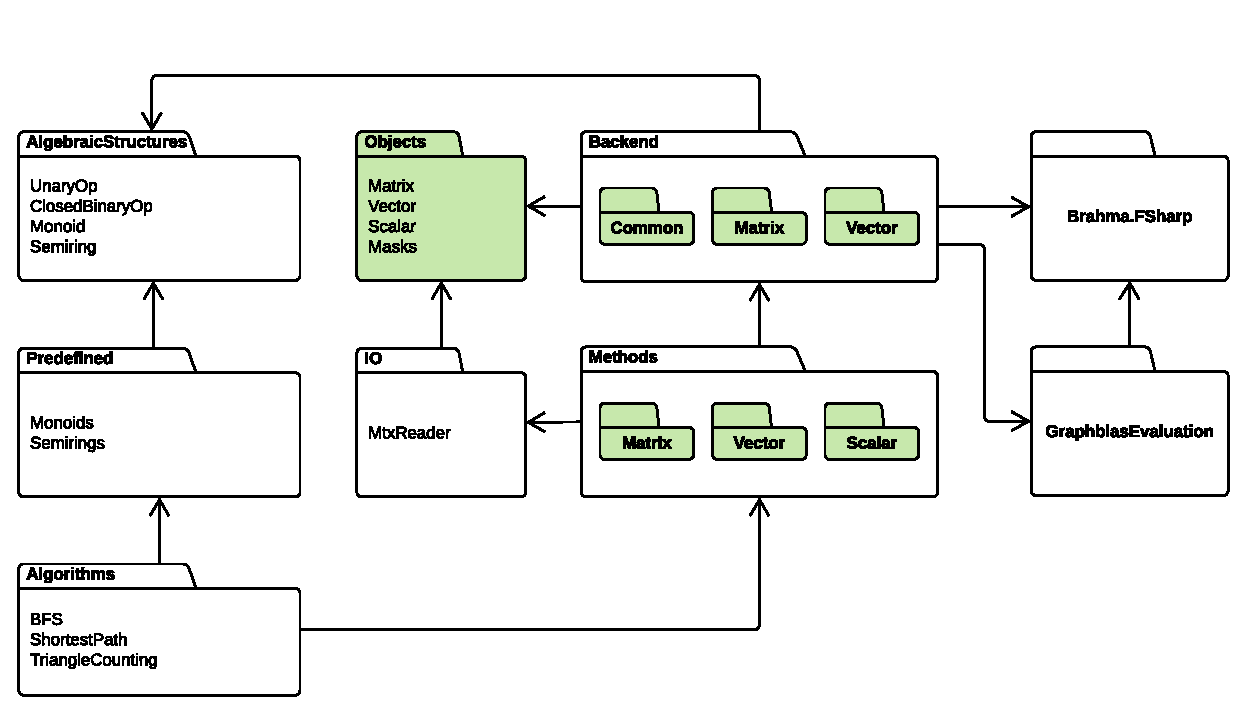
\includegraphics[scale=0.55]{architecture.pdf}}
\caption{Общая архитектура решения}
\end{figure}

\end{frame}

\begin{frame}{Описание решения}

Реализованные операции:
\begin{itemize}
    \item Поэлементное сложение матриц, векторов
    \begin{itemize}
        \item Слить массивы индексов в один с сохранением упорядоченности элементов
        \item Отметить повторяющиеся индексы в получившемся массиве
        \item Посчитать итоговую позицию каждого неповторяющегося индекса в получившемся массиве
        \item Перенести неповторяющиеся данные в результирующий массив индексов
    \end{itemize}
    \item Сокращение вектора при помощи аддитивной бинарной операции
    \item Запись значений в вектор через маску
    \begin{itemize}
        \item Профильтровать аргумент через маску
        \item Слить полученный вектор с вектором-целью
    \end{itemize}
\end{itemize}
    
\end{frame}

\begin{frame}{Сравнение с аналогом}

\begin{table}[h]
\center{}

\begin{tabular}{ | c | c | c | }
\hline
Название матрицы & Размер & Количество ненулевых элементов \\ \hline
luxembourg\_osm & 114599 & 119666 \\ \hline
belgium\_osm & 1441295 & 1549970 \\ \hline
wiki-Talk & 2394385 & 5021410 \\ \hline
cit-Patents & 3774768 & 16518948 \\ \hline
\end{tabular}

\caption{Матрицы, на которых производилось сравнение}
\label{matrices}
\end{table}


\begin{table}[h]
\center{}

\begin{tabular}{|c|c|c|}
\hline
& \multicolumn{2}{|c|}{Среднее время выполнения, мс} \\
\cline{2-3}
\raisebox{1.5ex}[0cm][0cm]{Название матрицы}
& SuiteSparse & GraphBLAS-sharp \\
\hline
luxembourg\_osm & 9.81 & 37.2 \\ \hline
belgium\_osm & 46.59 & 80.98 \\ \hline
wiki-Talk & 53.51 & 125.85 \\ \hline
cit-Patents & 263.47 & 504.51 \\ \hline
\end{tabular}

\caption{Результаты замеров сложения для библиотек GraphBLAS-sharp и SuiteSparse}
\label{graphblas-sharp}
\end{table}
    
\end{frame}

\begin{frame}{Сравнение с аналогом}
    
    \begin{table}[h]
    \center{}
    
    \begin{tabular}{ | c | c | c | }
    \hline
    Название матрицы & Размер & Количество ненулевых элементов \\ \hline
    luxembourg\_osm & 114599 & 119666 \\ \hline
    belgium\_osm & 1441295 & 1549970 \\ \hline
    wiki-Talk & 2394385 & 5021410 \\ \hline
    cit-Patents & 3774768 & 16518948 \\ \hline
    \end{tabular}
    
    \caption{Матрицы, на которых производилось сравнение}
    \label{matrices}
    \end{table}
    
    \begin{table}[h]
    \center{}
    
    \begin{tabular}{ | c | c | c | }
    \hline
    Название матрицы & Среднее время копирования данных, мс \\ \hline
    luxembourg\_osm & 6.57 \\ \hline
    belgium\_osm & 36.04 \\ \hline
    wiki-Talk & 85.52 \\ \hline
    cit-Patents & 353.38 \\ \hline
    \end{tabular}
    
    \caption{Результаты замеров времени копирования вспомогательных данных}
    \end{table}
    
\end{frame}

\begin{frame}{Выводы}
    
    \begin{itemize}
        \item Требуется снизить накладные расходы путём модифицирования библиотеки Brahma.FSharp
        \item С учётом переносимости и высокоуровневого интерфейса предлагаемое решение жизнеспособно
    \end{itemize}
    
\end{frame}

\begin{frame}
  \frametitle{Результаты}
  \begin{itemize}
    \item Разработана и реализована архитектура одномерной и двумерной маски, скаляра, а также разреженного вектора и матрицы, представленной в координатном формате
    \item Реализованы операции линейной алгебры с поддержкой OpenCL:
    \begin{itemize}
        \item Поэлементное сложение разреженных векторов и матриц, представленных в координатном формате
        \item Сокращение разреженного вектора при помощи аддитивной операции
        \item Запись в разреженный вектор через маску
    \end{itemize}
    \item Произведено сравнение с аналогом на примере поэлементного сложения
  \end{itemize}
\end{frame}

\end{document}